\documentclass[handout]{beamer}
\usepackage[utf8]{inputenc}
\usepackage{ stmaryrd }
\usepackage{tikz}

\usepackage{physics}
\usepackage{hyperref}
\usepackage{amsmath}
\usepackage{amsthm}
\usepackage{amssymb}
\usetheme{Madrid}
% \mode<presentation>{}
\usecolortheme{default}
\usepackage{mathtools}
\DeclarePairedDelimiter\ceil{\lceil}{\rceil}
\DeclarePairedDelimiter\floor{\lfloor}{\rfloor}
\newcommand{\cosec}{\operatorname{cosec}}

%------------------------------------------------------------
%This block of code defines the information to appear in the
%Title page
\title[MA109 Calculus-I] %optional
{MA109 Calculus-I}

\subtitle{D4-T6 Tutorial 3}

\author[Adish Shah] % (optional)
{Adish Shah}



\date[18th December 2021] % (optional)
{15th December 2021}



%End of title page configuration block
%------------------------------------------------------------



%------------------------------------------------------------
%The next block of commands puts the table of contents at the 
%beginning of each section and highlights the current section:

\AtBeginSection[]
{
  \begin{frame}
    \frametitle{Table of Contents}
    \tableofcontents[currentsection]
  \end{frame}
}
%------------------------------------------------------------


\begin{document}

%The next statement creates the title page.
\frame{\titlepage}

\begin{frame}
    \frametitle{{Lagrange's Mean Value Theorem (MVT)}}
	\begin{theorem}[MVT]
		Let $a < b$ and $f:[a, b] \to \mathbb{R}$ be a function such that\\
		(i) $f$ is continuous on $[a, b],$ and\\
		(ii) $f$ is differentiable on $(a, b).$\\
		Then there exists $c \in (a, b)$ such that $f'(c) = \dfrac{f(b) - f(a)}{b - a}.$
	\end{theorem}
\end{frame}

%---------------------------------------------------------
%Changing visivility of the text
\begin{frame}
\frametitle{1)}
\[f(x) = x^{3} - 6x+3\]
Let's find the stationary points of this polynomial.
\[f'(x) = 3x^{2}-6\]
\[\implies x = \pm \sqrt{2} \]
Now, \(f(-\sqrt{2}) = 4\sqrt{2}+3 > 0 \) and \(f(+\sqrt{2}) = -4\sqrt{2}+3 < 0 \). So by IVT, f has a root in 
$\left(-\sqrt{2},\sqrt{2}\right)$
\begin{itemize}
    \item<1-> \(f(x) \rightarrow -\infty\) as \(x \rightarrow -\infty \). By IVT, f has a root in $\left(-\infty,\sqrt{2}\right)$
    \item<2-> \(f(x) \rightarrow +\infty\) as \(x \rightarrow +\infty \). By IVT, f has a root in $\left(+\sqrt{2},\infty \right)$
\end{itemize}
Since f has at most three roots, all its root are real.
\end{frame}

\begin{frame}
\frametitle{4)}
Let the 3 distinct roots be $r_{1} < r_{2} < r_{3} $

By Rolle’s theorem $f'(x)$ has at
least two real roots, $x_{1}$ and $x_{2}$ such that $r_{1} < x_{1} < r_{2} $ and $r_{2} < x_{2} < r_{3} $.

Since $f'(x) = 3x^{2} + p$ this implies that $p < 0$, and $x_{1} = -\sqrt{\frac{-p}{3}}$,
$x_{2} = +\sqrt{\frac{-p}{3}}$

Now, $f''(x_{1} ) = 6x_{1} < 0 \implies$  f has a local maximum at $x=x_{1}$.
Similarly, f has a local minimum at $x=x_{2}$. 

This proves parts 1 and 2.
\end{frame}

\begin{frame}
    \frametitle{4) continued}
    Since the quadratic $f'(x)$ is negative between its roots $x_{1}$ and $x_{2}$ (so that f is decreasing over $[x_{1} , x_{2}]$) and
    f has a root $r_{2}$ in ($x_{1} , x_{2} $), we must have $f(x_{1} ) > 0$ and $f (x_{2} ) < 0$. 
    
    Further, 
    \[f(x_{1}) = q+ \sqrt{\frac{-4p^{3}}{27}},f(x_{2}) = q- \sqrt{\frac{-4p^{3}}{27}}\]

    \[f(x_{1})\times f(x_{2})< 0 \implies \frac{4p^{3}+27q^{2}}{27} < 0\]
    Hence proved.
    \end{frame}

\begin{frame}
\frametitle{5)}
To prove that $|\sin a - \sin b| \le |a - b|$ for all $a, b \in \mathbb{R}.$\\
Case 1. $a = b.$ We can clearly observe that the condition is satisfied.\\
Case 2. $a \neq b.$ Without loss of generality, we can assume that $a < b.$\\
As $f := \sin$ is continuous and differentiable on $\mathbb{R},$ there exists $c \in (a, b)$ such that $f'(c) = \dfrac{f(b) - f(a)}{b - a}.$ \hfill (By MVT)\\~\\
Also, we know that $|f'(c)| = |\cos c| \le 1.$\\~\\
Thus, we have it that $\left|\dfrac{f(b) - f(a)}{b - a}\right| \le 1.$\\~\\
\[\implies |\sin a - \sin b| \le |a - b| \]
\end{frame}

\begin{frame}
\frametitle{7)}
Assume that $f(0) \neq 0.$ Then, there are two possibilities.\\
	Case 1. $f(0) > 0.$\\
	The function $f$ satisfies the hypothesis of MVT, thus there must exist $c \in (-a, 0)$ such that $f'(c) = \dfrac{f(0) - f(-a)}{0 - (-a)} = \dfrac{f(0)}{a} + 1.$\\
	As $f(0) > 0$ and $a > 0,$ we get that $f'(c) > 1$ which contradicts the hypothesis.\\~\\
	Case 2. $f(0) < 0.$\\
	The function $f$ satisfies the hypothesis of MVT, thus there must exist $d \in (0, a)$ such that $f'(d) = \dfrac{f(a) - f(0)}{a - 0} =1 - \dfrac{f(0)}{a}.$\\
	As $f(0) < 0$ and $a > 0,$ we get that $f'(d) > 1$ which contradicts the hypothesis.\\~\\
\end{frame}





%-----------------------------------------------------
%Changing visivility of the text
\begin{frame}
\frametitle{8)}
    \begin{itemize}
      \item<(i)->(i) Assume that there exists such a function. We are given that $f''$ exists which implies that
                $f'$ must be continuous and differentiable everywhere.
                Since $f'(0) = f'(1)$, by Rolle's Theorem, $f''(c) = 0$ for some $c \in \left(0,1\right)$.
                This contradicts the condition that $f''(x) > 0$ for all $x \in \mathbb{R}$.
      \item<2-> (ii)Such a function exists. Example : $f:\mathbb{R} \rightarrow \mathbb{R}$ with $f(x) = \frac{x^{2}}{2}+x$.
      \item<3-> (iv) $e^{x}$ satisfies all the conditions given. Another possible function is :
      \begin{equation*} 
        f(x) = \begin{cases}
            \frac{1}{1-x} & x \le 0,\\
            1+x+x^{2} & x > 0.
        \end{cases}
    \end{equation*}

    \end{itemize}
\end{frame}

\begin{frame}
\frametitle{8) continued}
8(iii)
	Assume that such a function exists. Then, we are given that $f''$ exists. Thus, $f'$ must be continuous and differentiable everywhere.\\
	As $f''$ is nonnegative, $f'$ must be increasing everywhere. We are given that $f'(0) = 1.$ \\
	Thus, given any $c > 0,$ we know that $f'(c) \ge 1.$ \hfill (1)\\
	Let $x \in (0, \infty).$ By MVT, we know that there exists $c \in (0, x)$ such that $f'(c) = \dfrac{f(x) - f(0)}{x - 0}.$ \\ Thus, by (1), we have it that $f(x) - f(0) \ge x$ for all positive $x.$ \\
	This contradicts that $f(x) \le 100$ for all positive $x.$ 
\end{frame}


\begin{frame}
    \frametitle{9)}
    \[f(x) = \left\{\begin{array}{l r}
		1 - 12x - 3x^2  & \text{if } x \le 0\\
		1 + 12x - 3x^2	& \text{if } x > 0
	\end{array}
	\right.\]
	As $f:[-2, 5] \to \mathbb{R}$ is continuous, we have it that the absolute extrema of $f$ on $[a, b]$ is attained either at a critical point of $f$ or at an end-point of $[a, b].$\\
	An interior point $c$ of the domain is called a critical point of $f$ if either $f$ is not differentiable at $c,$ or if $f$ is differentiable at $c$ and $f'(c) = 0.$\\
	$0$ is a critical point as $f$ is not differentiable at $0.$ Moreover, $0$ is the only point at which $f$ is not differentiable.\\
	For $x < 0,$ we get the derivative of $f$ as $f'(x) = -12 - 6x = -6(x + 2).$ Thus, no negative number in the domain is a critical point. (Note that $-2$ is \textbf{not} an interior point of the domain.)
\end{frame}

\begin{frame}
    \frametitle{9) continued}
	For $x > 0,$ we get the derivative as $f'(x) = 12 - 6x = 6(2 - x).$ Thus, $2$ is a critical point of $f.$ (Note that $2$ \textbf{is} an interior point of the domain.)\\~\\
	To summarise,\\
	Critical points of $f:$ $0, 2.$ End-points of $[-2, 5]:$ $-2, 5.$\\
	\begin{center}
		\begin{tabular}{|c| c c c c|}
		\hline
		x & 0 & 2 & -2 & 5\\
		f(x) & 1 & 13 & 13 & -14 \\
		\hline
		\end{tabular}
	\end{center}
	$\therefore f$ attains its global maximum $13$ at $2$ as well as $-2,$ and its global minimum $-14$ at $5.$
\end{frame}
%---------------------------------------------------------
%Changing visivility of the text
\begin{frame}
    \frametitle{10)}
	\begin{figure}
		\centering
		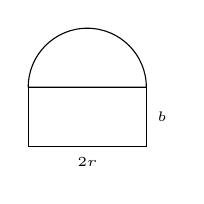
\begin{tikzpicture}
			\def \r{0.75}
			\def \b{0.75}
			\draw[] (0, \b) -- (0, 0) -- (2*\r, 0) -- (2*\r, \b);
			\draw[] (0, \b) -- (2*\r, \b) arc(0:180:\r);
			\node[] at (\r, - 0.2) {\tiny $2r$}; 
			\node[] at (2*\r + 0.2, \b/2) {\tiny $b$}; 
		\end{tikzpicture}
	\end{figure}
Given perimeter of the window is to be $p$.
\[p = 2b+2r+\pi r = 2b + (\pi+2)r \]
Let $l(r, b)$ denote the amount of light that enters through the window for $r$ and $b$ specified in the diagram.\\
	We know that $l(r, b) = k(2rb) + \left(\frac{k}{2}\right)(\frac{\pi r^2}{2}).$ Where $k$ is some positive constant.\\
    Rewriting b in terms of p, we get 
    $L(r) = l\bigg(r, \frac{1}{2}\big(p - (2 + \pi)r\big)\bigg) = k\left[r(p - (2 + \pi)r) + \frac{\pi r^2}{4}\right] = k \left[pr - 2r^2 - \frac{3\pi r^2}{4}\right].$\\
\end{frame}

\begin{frame}
    \frametitle{10) continued}
    As the above is defined for $(0, \infty)$ and is differentiable everywhere, we only need to check where the derivative is zero.\\~\\
	$L'(r) = k\left[p - 4r - \frac{3\pi r}{2}\right] = k\left[p - \left(\frac{8 + 3\pi}{2}\right)r\right] .$\\
	$\therefore L'(r) = 0 \implies r = \dfrac{2p}{8 + 3\pi}.$\\~\\
	You can verify that for this value of $r,$ $L''(r)$ is negative. \\~\\
	$b$ can now be calculated as we know the relation between $b, p$ and $r.$\\
	It comes out to be $\dfrac{1}{2}\left(\dfrac{4 + \pi}{8 + 3\pi}\right)p.$
\end{frame}

%---------------------------------------------------------

%Example of the \pause command
% \begin{frame}
%  in this slide \pause

% the text will be sounds partially visible \pause

% And finally everything will be there
% \end{frame}
%---------------------------------------------------------


% \section{Background of Shor's Algorithm}
% %---------------------------------------------------------
% \begin{frame}
% \frametitle{Background}
%     Let us look at the background of Shor's algorithm
%     \begin{itemize}
%       \item<1-> Quantum Algorithm, to find the prime factors of any given integer N
%       \item<2-> Named after a mathematician, Peter Shor who formulated the algorithm in 1994.
%       \item<3-> This algorithm cam factor a number N in $O((logN)^3)$ time and $O(logN)$ space.
%       \item<4-> This demonstrates that an integer factorization can be done on a quantum computer in polynomial time. 
%     \end{itemize}
% \end{frame}
% \begin{frame}
% \frametitle{RSA}
%     RSA is a popular encyrption technique that uses a public key N which is the product of two large prime numbers.
%     \begin{itemize}
%       \item<1-> One way to crack RSA encyrption is by factoring N, but, with classical algorithms, factoring becomes increasingly time-consuming as N grows larger.
%       \item<2-> More specifically, there is \textbf{no classical algorithm} known that can factor a number N in polynomial time.
%     \end{itemize}
%   \end{frame}
% \section{Grover's algorithm}

% \begin{frame}
%   Like many other quantum algorithms, Shor's algorithm is probabilistic. \pause
%   This means that it will give the correct answer with high probability, and the probability of success can be increased by performing more iterations.
% \end{frame}

% \begin{frame}
% Discrete Fourier Transform acts on a vector of complex numbers, $x_{0},x_{1},\dots , x_{N-1}$. of fixed length N, and outputs another vector of complex numbers,$y_{0},y_{1},\dots , y_{N-1}$ given by :
% $$y_{k} = \frac{1}{\sqrt{N}} \sum_{j=0}^{N-1}x_{j}e^{2 \pi ijk/N}$$ \pause
% The quantum Fourier Transform is defined in a similar way. The QFT on an orthonormal basis of vectors $\ket{0},\ket{1},\dots,\ket{N-1}$ is defined to be a linear operator with the following action on the basis state:
% $$\ket{j} \shortrightarrow  \frac{1}{\sqrt{N}} \sum_{j=0}^{N-1} \ket{k}e ^{2 \pi ijk/N}$$ \pause
% This can also be seen as :
% $$ \sum_{j=0}^{N-1} x_{j} \ket{j} = \sum_{k=0}^{N-1}y_{k} \ket{k}$$

% \end{frame}
%---------------------------------------------------------
% %Highlighting text
% \begin{frame}
% \frametitle{Introduction to Grover's algorithm}

% % In this slide, some important text will be
% % \alert{highlighted} because it's important.

% % Please, don't abuse it.

% % \begin{block}{Remark}
% % Sample text
% % \end{block}

% % \begin{alertblock}{Important theorem}
% % Sample text in red box
% % \end{alertblock}

% % \begin{examples}
% % Sample text in green box. The title of the block is ``Examples".
% % \end{examples}
% % \end{frame}

% Let us now look at another classical computing task that can be sped up using the superposition principle. \pause

% Our aim is to solve the needle in a haystack problem where we have to search for an element which satisfies a particular property, and it lies in a haystack of $N$ elements. \pause

% Classically, this would take $O(N)$ steps to do this task, but Grover's algorithm allows us to do it in $O(\sqrt{N})$ steps.
% \end{frame}

% \begin{frame}
%   \frametitle{Problem statement}
%   \begin{block}{Problem}
%     Suppose f(x) is a function from $\{0,1,\dots\}$ to $\{0,1\}$. f(a) = 1, only for one value of a. Find a. Assume that $N = 2^{n}$. This way you can work with n qubits.
%   \end{block}  
% \end{frame}

% \begin{frame}
%   \frametitle{Solution - Grover's Method}
%   \begin{center}
%     Let us define two new state vectors : \pause 
%   \end{center}
%   $$ \ket{\Psi_{0}} = \sum_{i=0}^{N-1} \frac{\ket{i}}{\sqrt{N}} $$ \pause
%   $$ \ket{e} = \sum_{i=0, i \neq a}^{N-1} \frac{\ket{i}}{\sqrt{N-1}} $$ \pause 
  
%   \begin{center}
%     Our goal is to ensure that we obtain $\ket{a}$ in the end. Notice that \pause
%     $$     \ket{\Psi_{0}} = \frac{\sqrt{N-1}\ket{e}+ \ket{a}}{\sqrt{N}}    $$ 
%     Thus $\ket{\Psi_{0}}$ lies in the subspace spanned by $\ket{e}$ and $\ket{a}$
%   \end{center}

% \end{frame}
% \begin{frame}
%   Note that, $\ket{\Psi_{0}}$ will be closer to $\ket{e}$ than $\ket{a}$. \pause
% %   \begin{figure}[htp]
% %     \centering
% %     \includegraphics[scale = 0.5]{grover.png}
% %   \end{figure}
% \end{frame}
% %---------------------------------------------------------
% \begin{frame}
%   We aim to take a vector $\ket{\Psi}$ which will initially be equal to $\ket{\Psi_{0}}$. \pause


%   Rotate it so that it ends up getting close to $\ket{a}$ \pause


%   First reflect $\Psi$ about $\ket{e}$ and then about $\ket{\Psi_{0}}$.
%   Reflecting about $\ket{e}$ can be considered as an oracle that performs the operation O
%   $$ \ket{x} \shortrightarrow (-1)^{f(x)}\ket{x}$$ \pause
%   The way to achieve this is to take an oracle that performs the operation 
%   $$ \ket{x}\ket{y} \shortrightarrow \ket{x} \ket{y \oplus f(x)}$$
%   Let $\ket{y}$ = $\frac{\ket{0}-\ket{1}}{\sqrt{2}}$ \pause
%   If x = a, $$\ket{x} \ket{y} \shortrightarrow - \ket{x} \ket{y} $$
%   Else, state will be preserved.

% \end{frame}

% \begin{frame}
%   \begin{block}{Remark}
%     It turns out mathematically, that Grover's operator G is 
%   $$G = (2\ket{\Psi_{0}}\bra{\Psi_{0}}- I)O$$ 
%   \end{block}
%   \pause 
% %   \begin{figure}[htp]
% %     \centering 
% %     \includegraphics[scale = 0.3]{Screenshot from 2021-07-19 22-30-03.png}
% %   \end{figure} \pause
%   Let $\ket{\Psi_{0}}$ make an angle $\theta$ with $\ket{e}$ in the two dimension subspace. Then,
%   $$ sin(\theta) = \frac{1}{\sqrt{N}} $$
% \end{frame}  
% %---------------------------------------------------------
% %Two columns
% \begin{frame}
  
% \begin{block}{Remark}
%   By induction, 
%   $$G^{k} \ket{\Psi_{0}} = cos((2k+1)\theta)\ket{e} + sin((2k+1)\theta)\ket{a}$$
% \end{block}
%  \pause 
% Applying G successively on $\ket{\Psi_{0}}$ rotates the vector by an angle $2\theta$ \pause 


% Goal is to make the angle between $\ket{\Psi}$ and $\ket{a} \le \theta$ \pause 


% Probability of collapsing will be $\ge cos(\theta) = \frac{\sqrt{N-1}}{\sqrt{N}}$ 

% \end{frame}
% \begin{frame}
%   \frametitle{Conclusion}
%   How many operations of G do we need though? \pause 
%   Clearly we require [$\frac{\pi}{4\theta}$] applications of G. As $\theta \ge sin(\theta) = \frac{1}{\sqrt{N}}$,
%   $$[\frac{\pi}{4\theta}] \le \frac{\pi \sqrt{N}}{4}$$ \pause 
%   Thus we need only $O(\sqrt{N})$ operations to achieve the task with probability $\ge \frac{\sqrt{N-1}}{\sqrt{N}} $

% \end{frame}
%---------------------------------------------------------


\end{document}